% Quick repository for all APA gap crossing figures

\graphicspath{{AppendixAPAGap/Figs/}}

%----------------------------------------------------------------------------------------------------------------------------------------------------------------------------
\chapter{APA Gap-Crossing Muons: Gap Measurements}\label{appen:APAGap}

This appendix contains all figures used to make measurement of the gaps between the APA frames in the 35-ton experiment, as discussed in Section~\ref{sec:APAGapCrossing} and presented in Table~\ref{tab:APAOffsets}.  The method used is described in detail in Section~\ref{sec:MeasuringAPAGaps}.

The following pages contain the information for each of the four gaps in the long drift region in the 35-ton detector: DV1/DV3 (Figure~\ref{fig:AppendixTPC1TPC3}), DV1/DV5 (Figure~\ref{fig:AppendixTPC1TPC5}), DV3/DV7 (Figure~\ref{fig:AppendixTPC3TPC7}) and DV5/DV7 (Figure~\ref{fig:AppendixTPC5TPC7}).  The top figure shows the initial measurement of the $z$-offset, with the double-peak effect and the associated initial extraction of a $z$-offset; the centre figure shows the measurement of the $x$-offset after correcting for the initial $z$-offset estimate; and the bottom figure shows the measurement of the $z$-offset after correcting for the determined $x$-offset.  In each case, the initial $z$-offset is found by fitting a parabola between the peaks except for the DV3/DV7 case.  In this instance, the number of tracks in the sample is too low to make meaningful measurements of this effect and instead a coarse binning is chosen to mask the peaks and a Gaussian fit is used on the resulting distribution.  As is evident from the following figures, this works reasonably well in the case of small sample size.

\begin{figure}
  \centering
  \begin{subfigure}[t]{\linewidth}
    \centering
    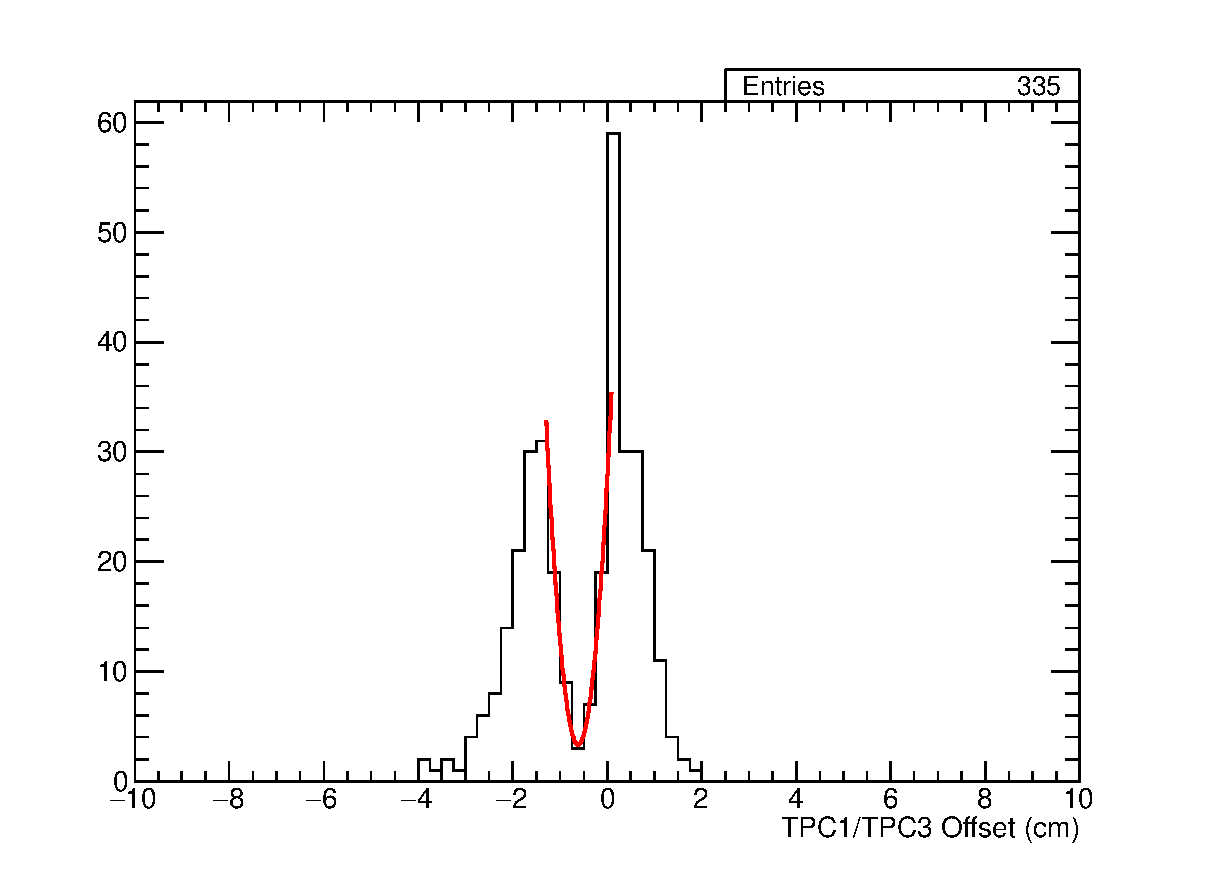
\includegraphics[width=9cm]{TPC1TPC3Gap.eps}
    \caption{Initial $z$-offset}
    \label{fig:AppendixTPC1TPC3Gap}
  \end{subfigure}
  \vfill
  \begin{subfigure}[t]{\linewidth}
    \centering
    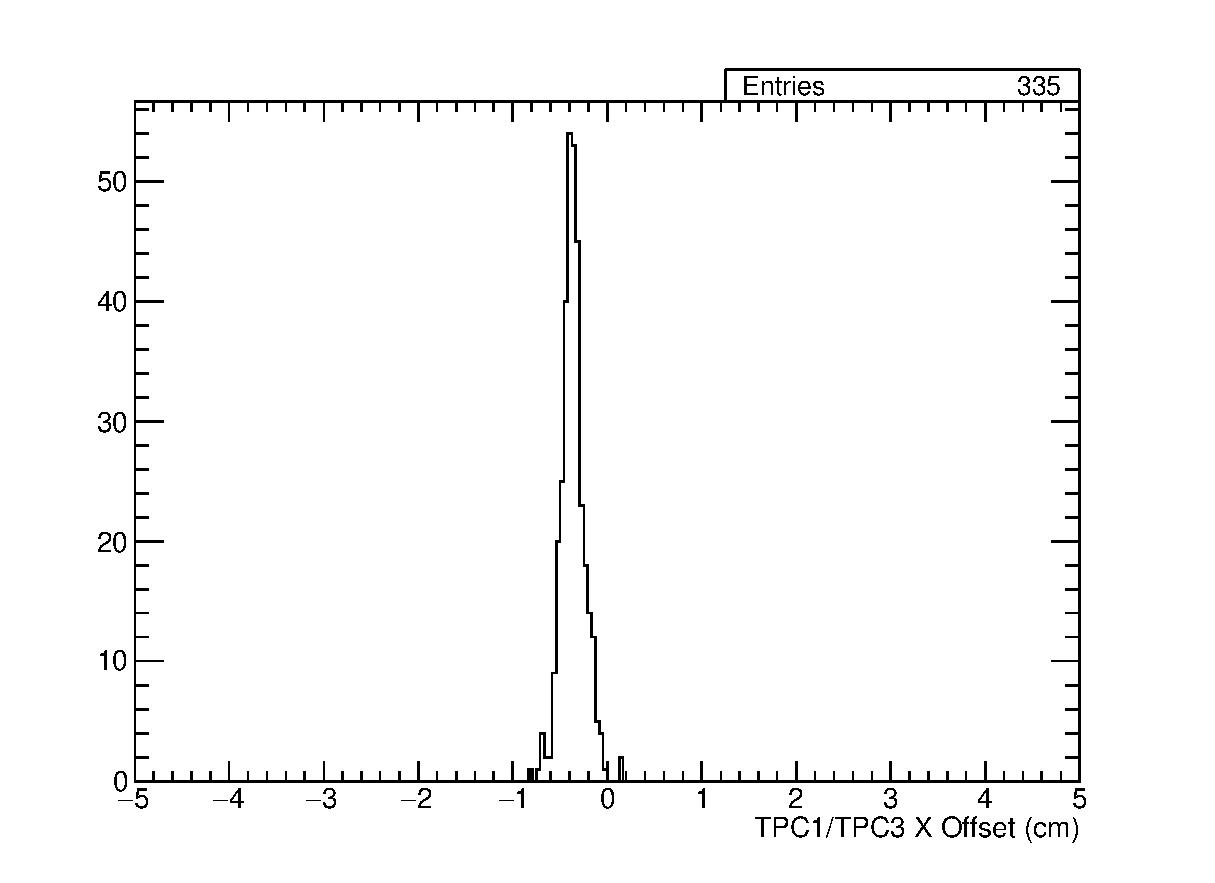
\includegraphics[width=9cm]{TPC1TPC3XOff.eps}
    \caption{$x$-offset}
    \label{fig:AppendixTPC1TPC3XOff}
  \end{subfigure}
  \vfill
  \begin{subfigure}[t]{\linewidth}
    \centering
    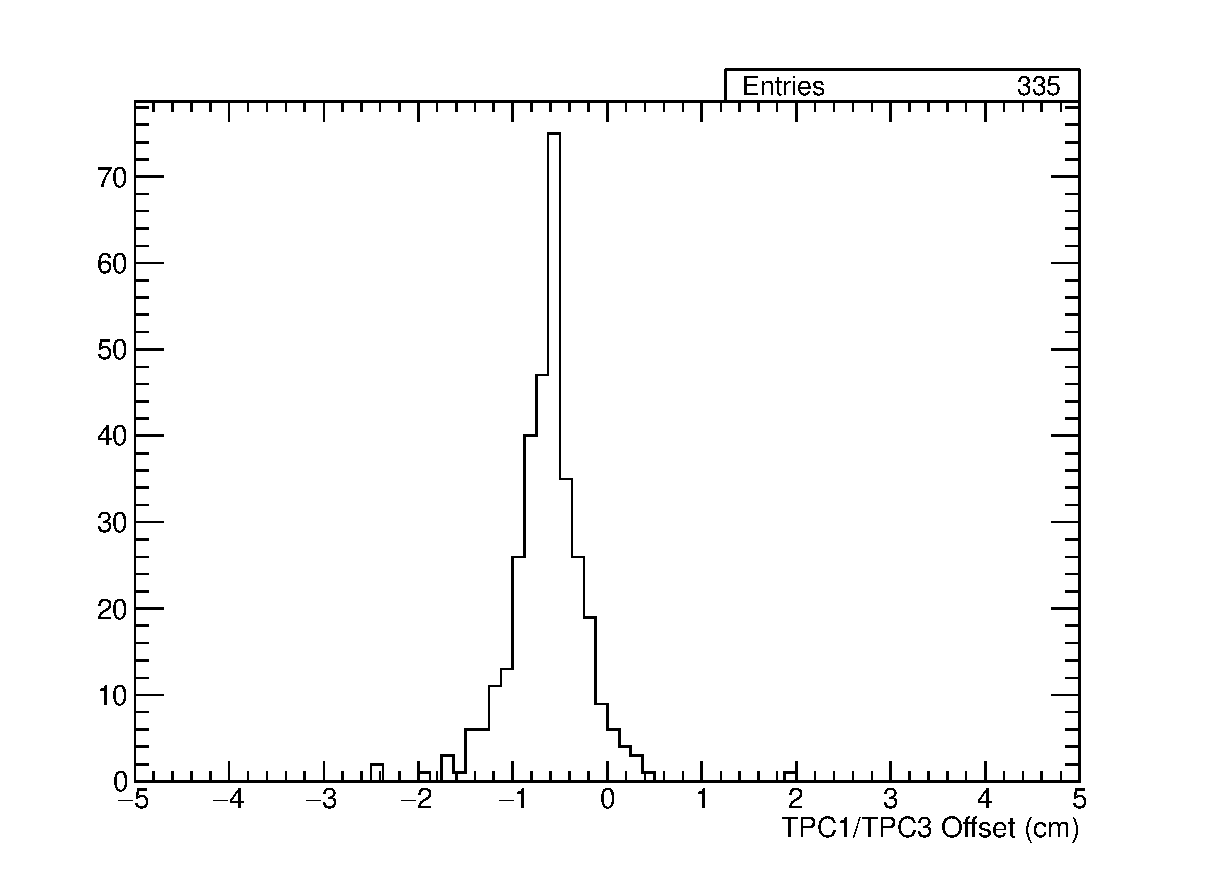
\includegraphics[width=9cm]{TPC1TPC3ZOff.eps}
    \caption{$z$-offset}
    \label{fig:AppendixTPC1TPC3ZOff}
  \end{subfigure}
  \caption[Demonstration of the measurements of the $x$- and $z$-offsets in the 35-ton DV1/DV3 gap.]{DV1/DV3 gap.}
  \label{fig:AppendixTPC1TPC3}
\end{figure}


\begin{figure}
  \centering
  \begin{subfigure}[t]{\linewidth}
    \centering
    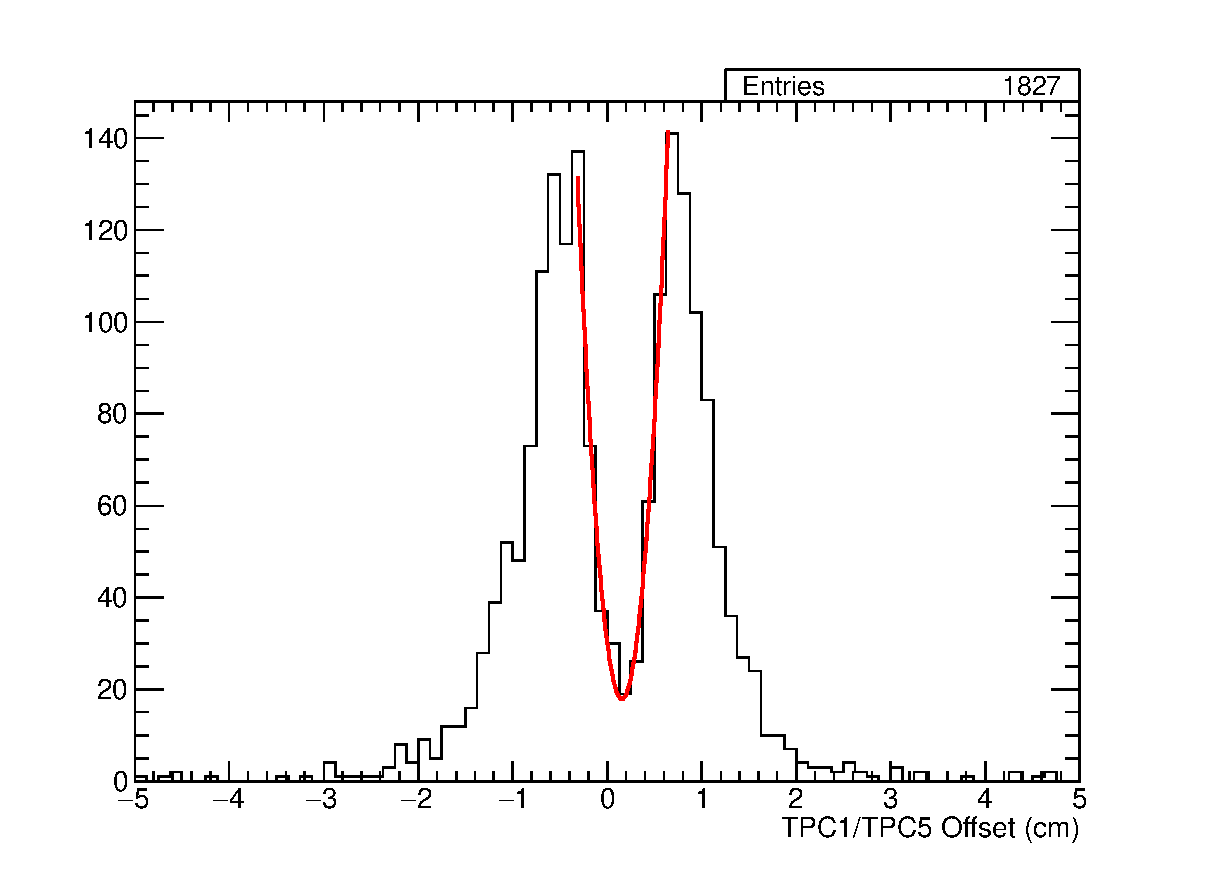
\includegraphics[width=9cm]{TPC1TPC5Gap.eps}
    \caption{Initial $z$-offset}
    \label{fig:AppendixTPC1TPC5Gap}
  \end{subfigure}
  \vfill
  \begin{subfigure}[t]{\linewidth}
    \centering
    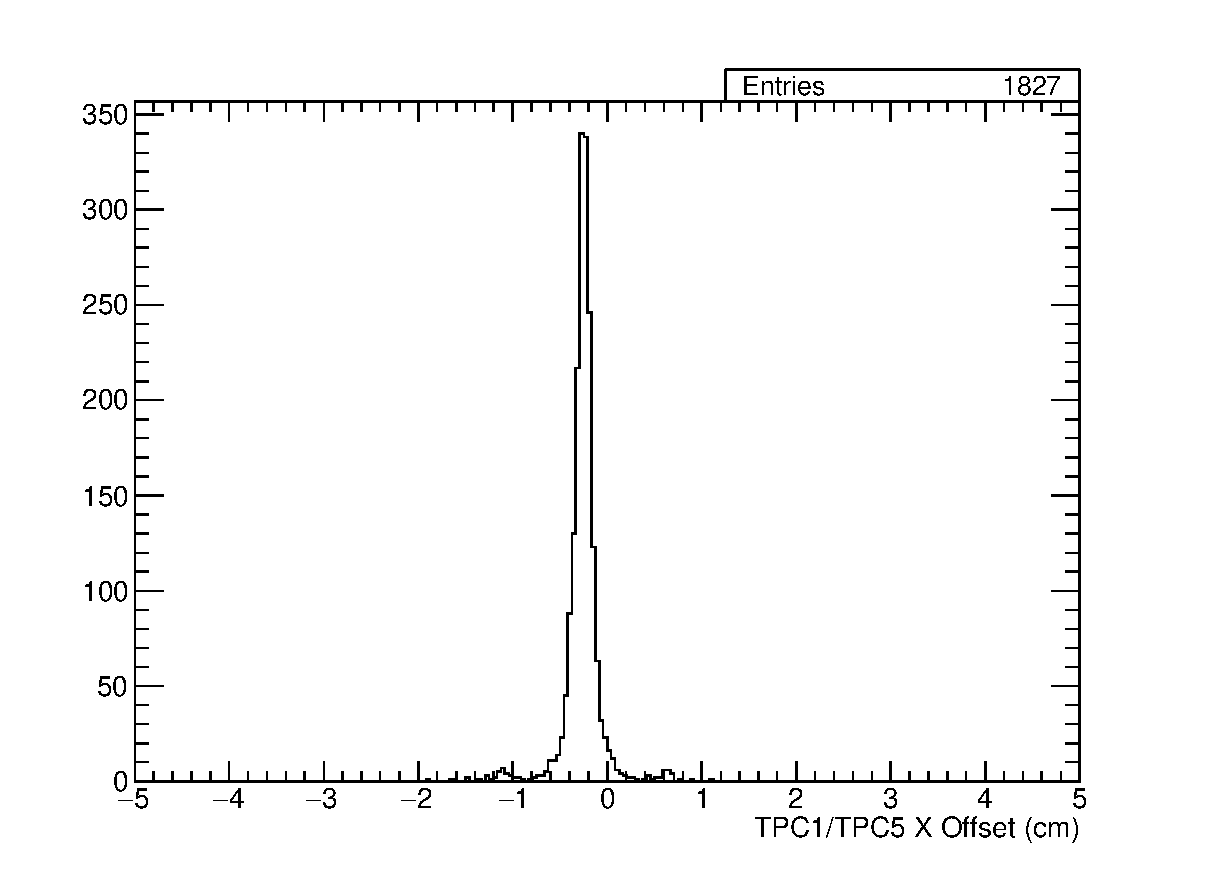
\includegraphics[width=9cm]{TPC1TPC5XOff.eps}
    \caption{$x$-offset}
    \label{fig:AppendixTPC1TPC5XOff}
  \end{subfigure}
  \vfill
  \begin{subfigure}[t]{\linewidth}
    \centering
    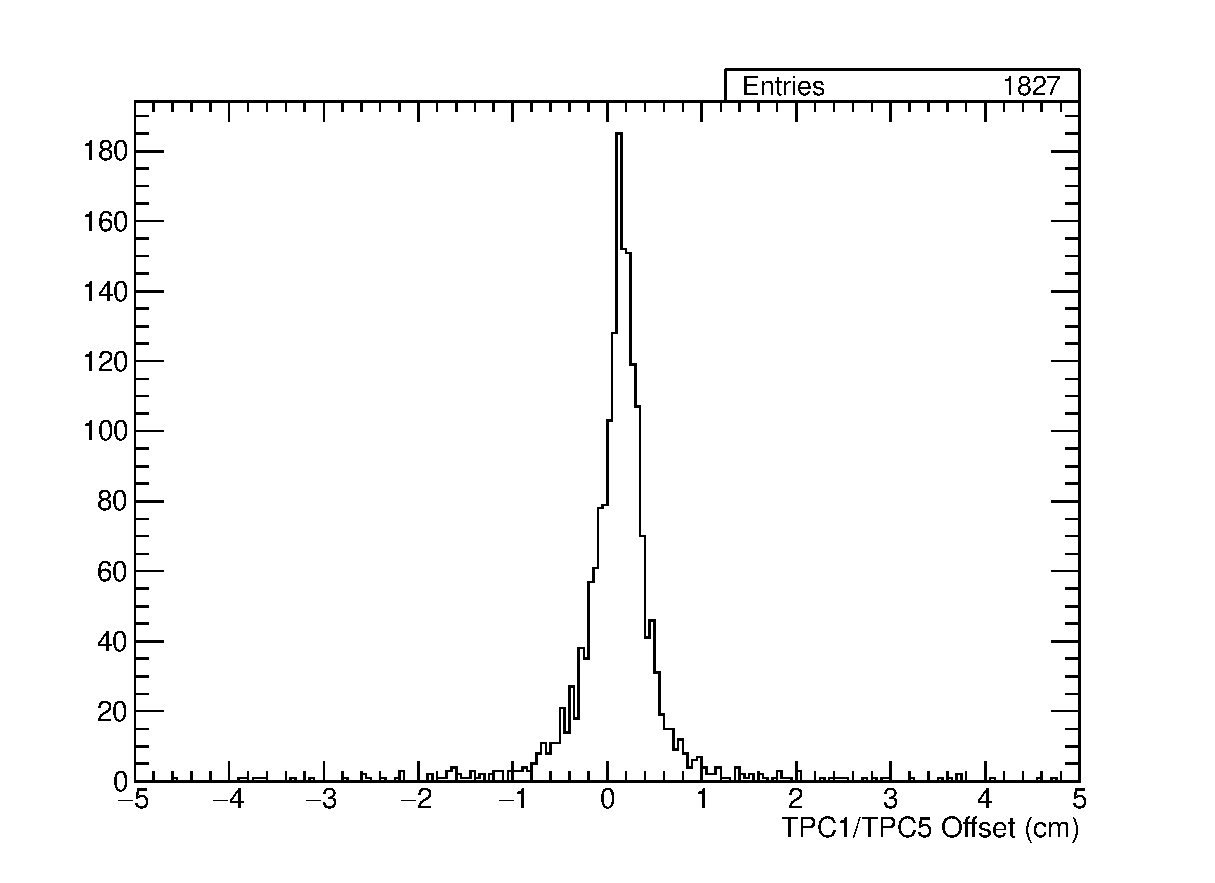
\includegraphics[width=9cm]{TPC1TPC5ZOff.eps}
    \caption{$z$-offset}
    \label{fig:AppendixTPC1TPC5ZOff}
  \end{subfigure}
  \caption[Demonstration of the measurements of the $x$- and $z$-offsets in the 35-ton DV1/DV5 gap.]{DV1/DV5 gap.}
  \label{fig:AppendixTPC1TPC5}
\end{figure}


\begin{figure}
  \centering
  \begin{subfigure}[t]{\linewidth}
    \centering
    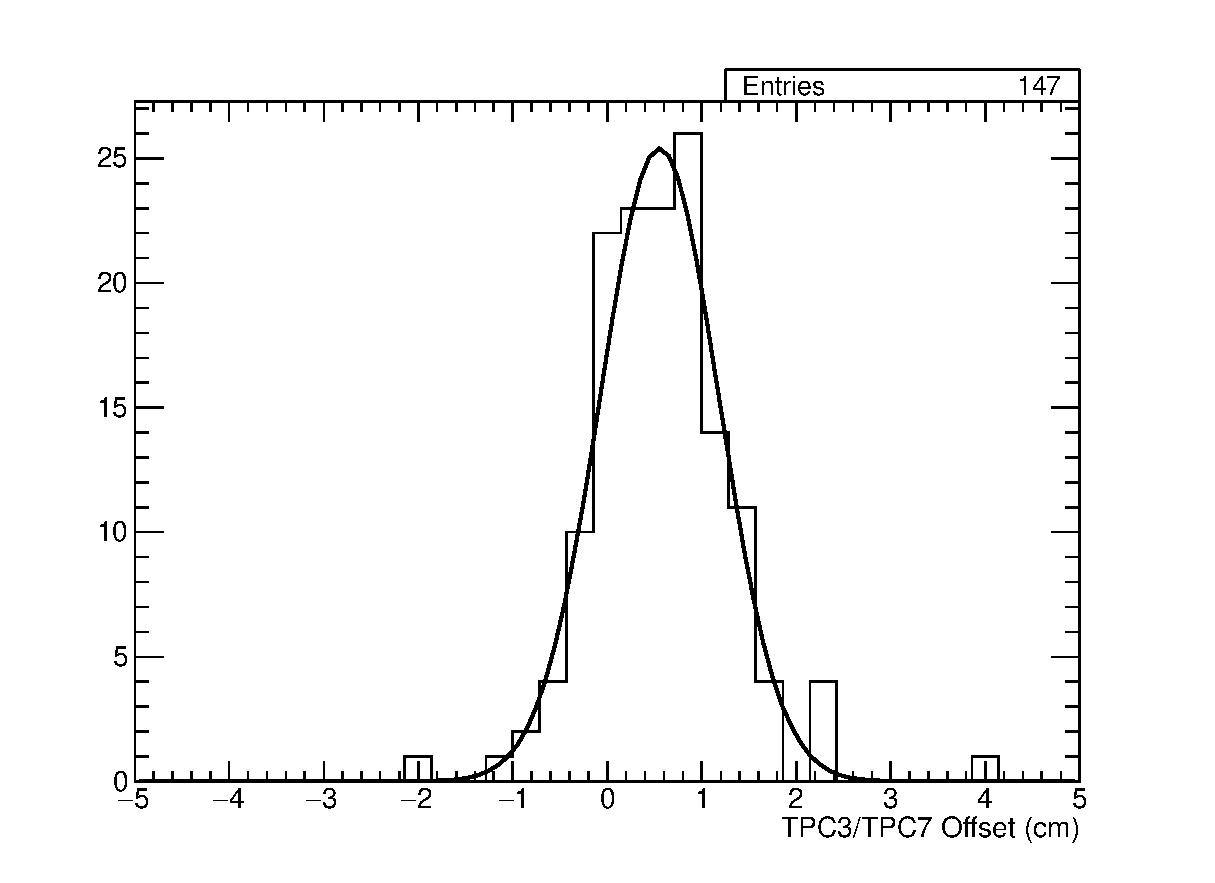
\includegraphics[width=9cm]{TPC3TPC7Gap.eps}
    \caption{Initial $z$-offset}
    \label{fig:AppendixTPC3TPC7Gap}
  \end{subfigure}
  \vfill
  \begin{subfigure}[t]{\linewidth}
    \centering
    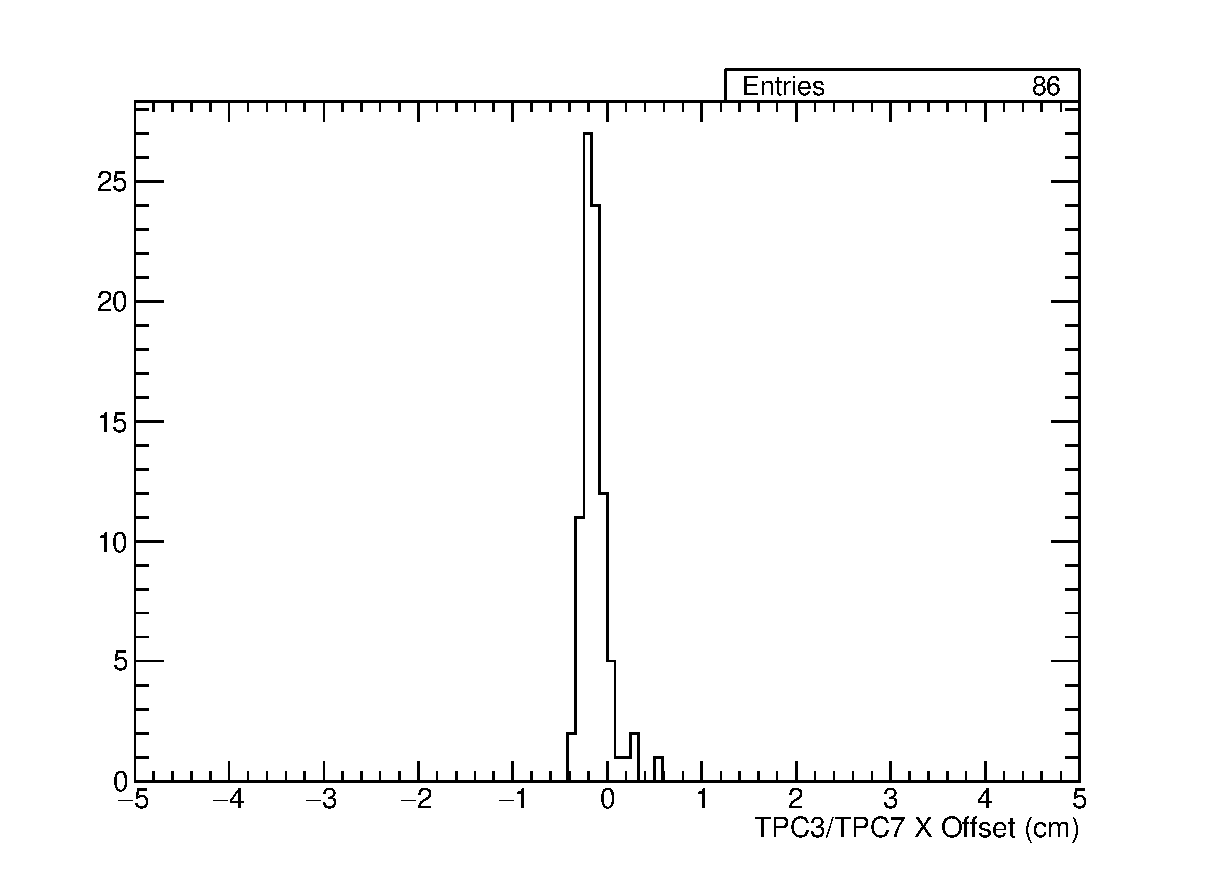
\includegraphics[width=9cm]{TPC3TPC7XOff.eps}
    \caption{$x$-offset}
    \label{fig:AppendixTPC3TPC7XOff}
  \end{subfigure}
  \vfill
  \begin{subfigure}[t]{\linewidth}
    \centering
    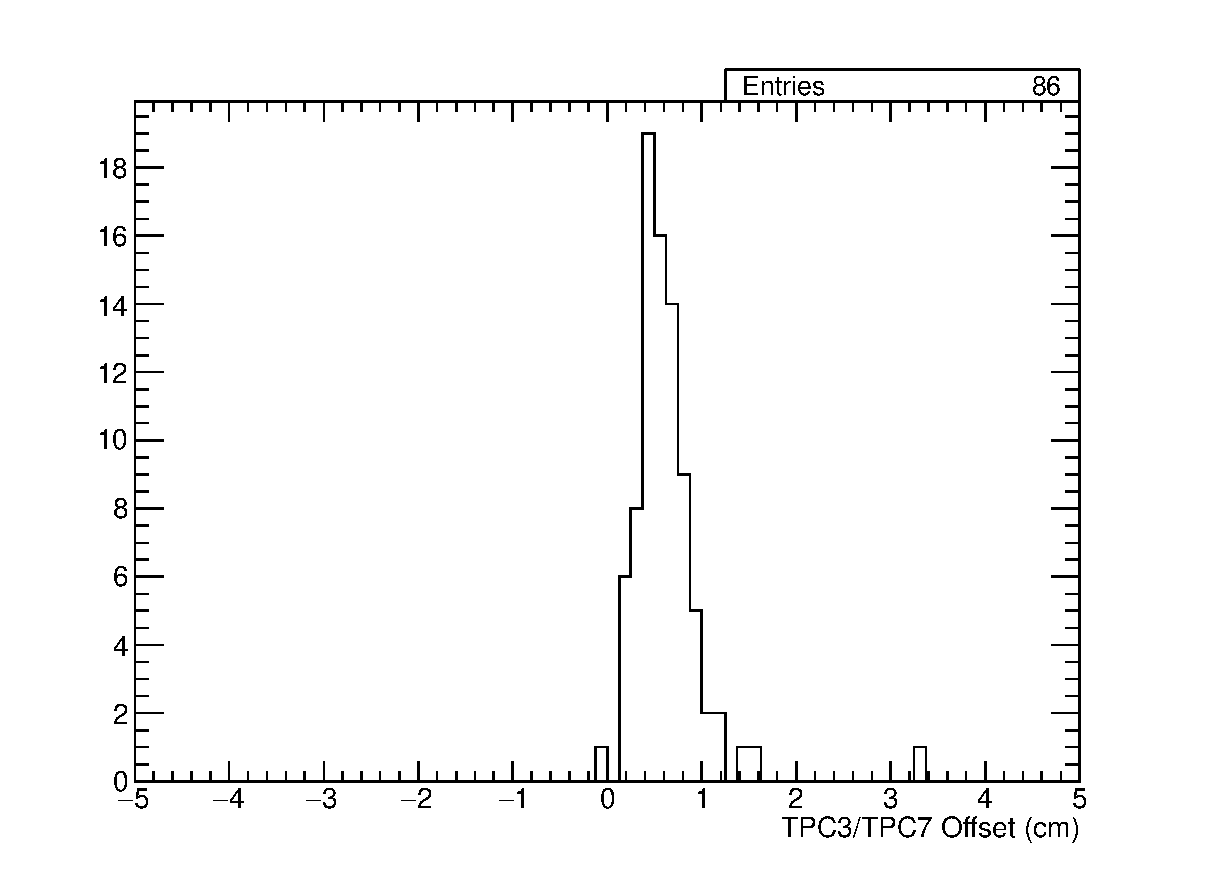
\includegraphics[width=9cm]{TPC3TPC7ZOff.eps}
    \caption{$z$-offset}
    \label{fig:AppendixTPC3TPC7ZOff}
  \end{subfigure}
  \caption[Demonstration of the measurements of the $x$- and $z$-offsets in the 35-ton DV3/DV7 gap.]{DV3/DV7 gap.}
  \label{fig:AppendixTPC3TPC7}
\end{figure}


\begin{figure}
  \centering
  \begin{subfigure}[t]{\linewidth}
    \centering
    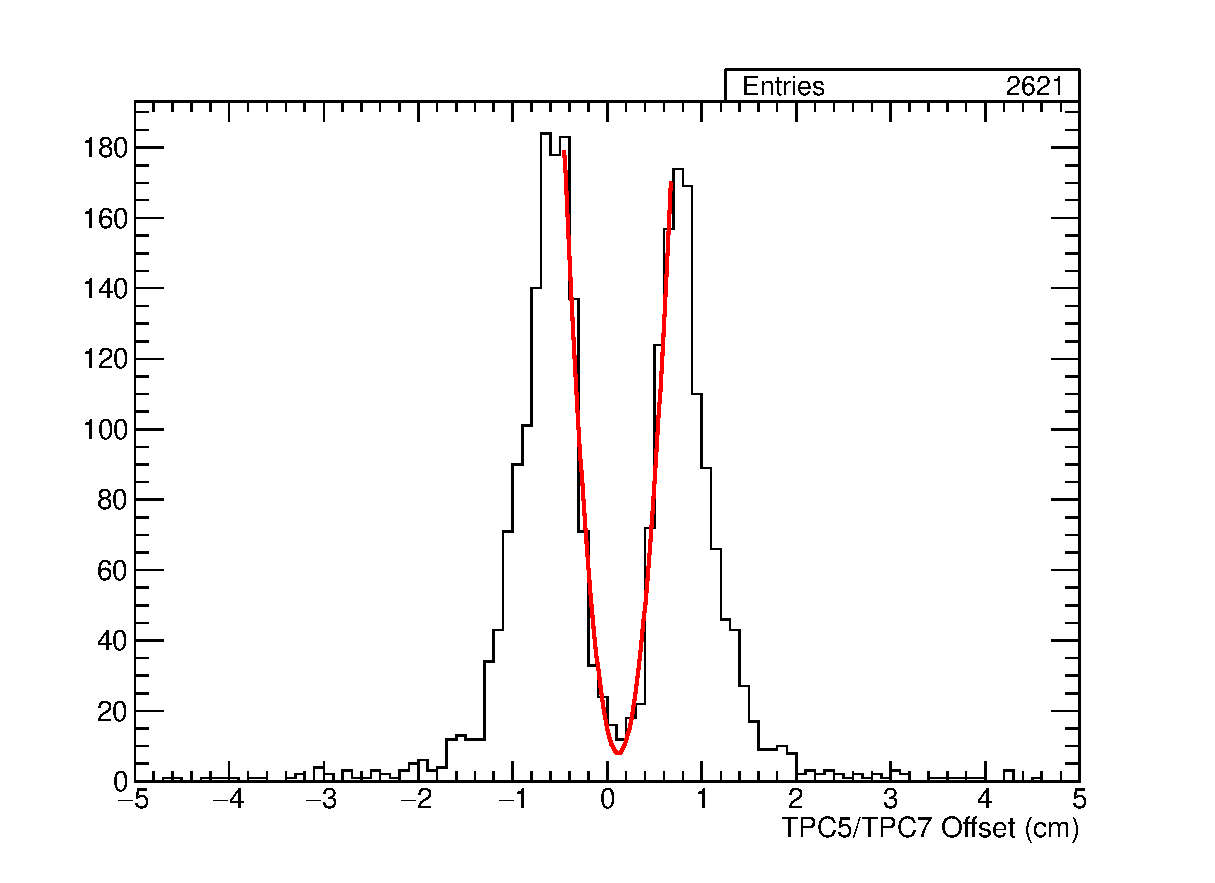
\includegraphics[width=9cm]{TPC5TPC7GapFit.eps}
    \caption{Initial $z$-offset}
    \label{fig:AppendixTPC5TPC7Gap}
  \end{subfigure}
  \vfill
  \begin{subfigure}[t]{\linewidth}
    \centering
    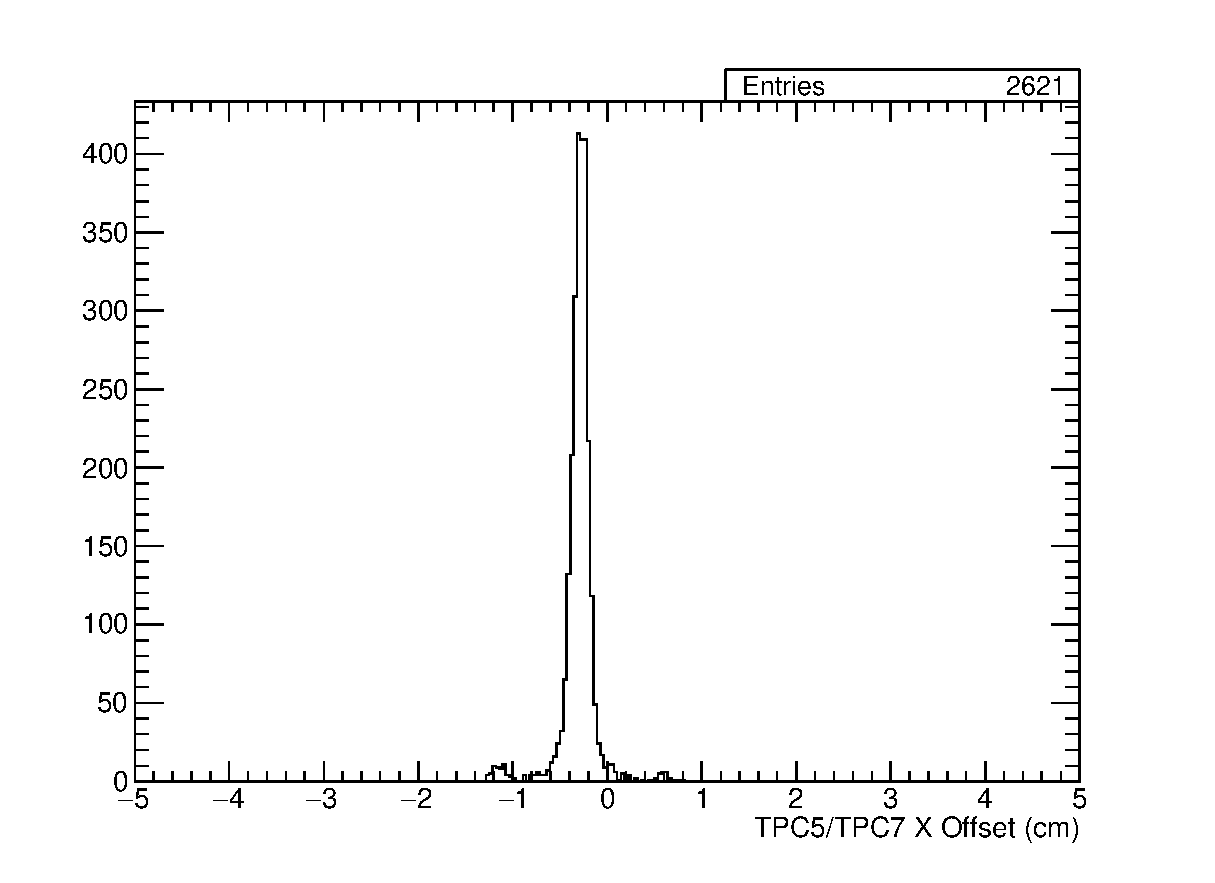
\includegraphics[width=9cm]{TPC5TPC7XOff.eps}
    \caption{$x$-offset}
    \label{fig:AppendixTPC5TPC7XOff}
  \end{subfigure}
  \vfill
  \begin{subfigure}[t]{\linewidth}
    \centering
    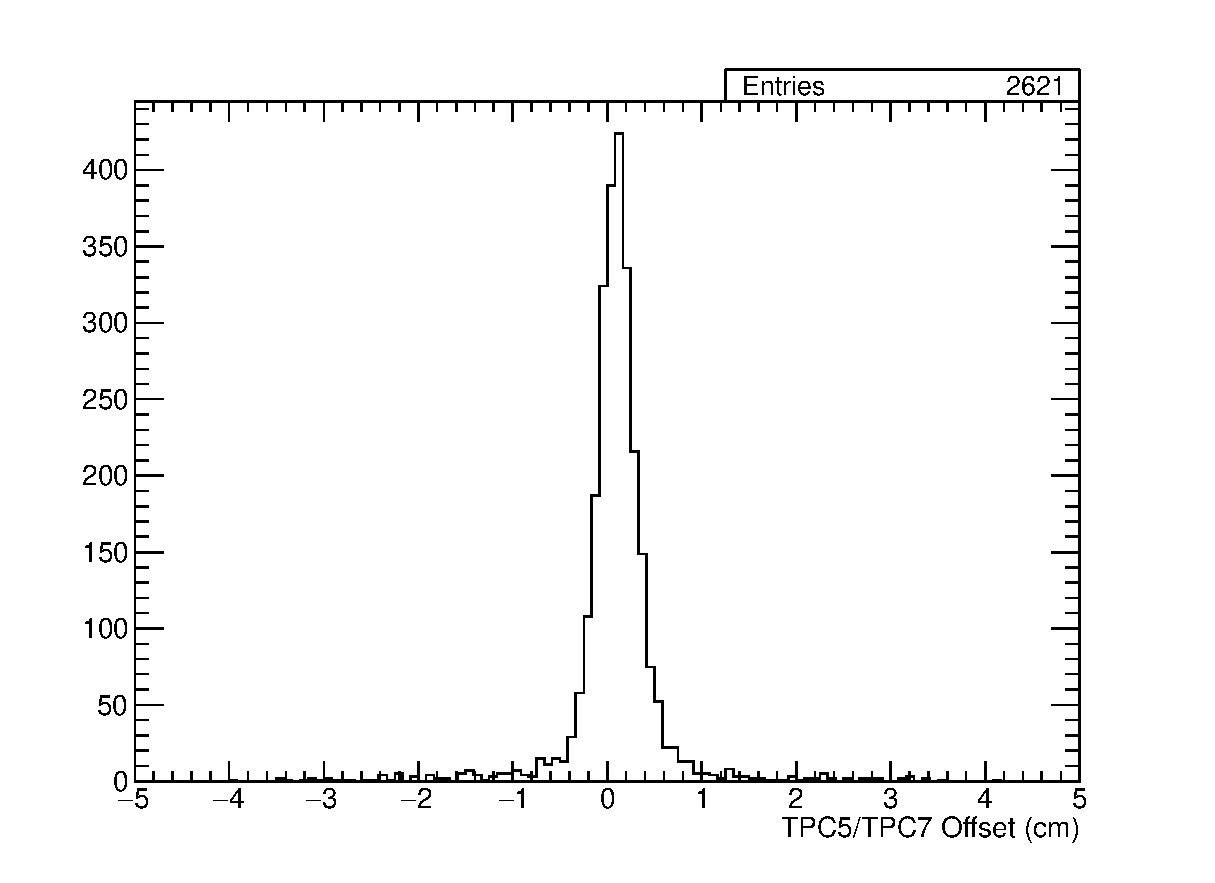
\includegraphics[width=9cm]{TPC5TPC7ZOff.eps}
    \caption{$z$-offset}
    \label{fig:AppendixTPC5TPC7ZOff}
  \end{subfigure}
  \caption[Demonstration of the measurements of the $x$- and $z$-offsets in the 35-ton DV5/DV7 gap.]{DV5/DV7 gap.}
  \label{fig:AppendixTPC5TPC7}
\end{figure}
